
% [handout] weglassen für animationen
\documentclass[handout]{beamer}

\usepackage[utf8]{inputenc}
\usepackage{graphicx}
\usepackage{geometry}
\usepackage{tikz}
\usepackage{hyperref}
\usepackage{textcomp}


\usetheme[numbering=counter, progressbar=frametitle, block=fill]{metropolis}
\graphicspath{ {res/} }

\title{Linux: Grundkurs}
\subtitle{Eine Einführung in den KDE-Desktop}
\author{Paul Seidel}
\date{02.12.2023} %may change \today
\institute{ZKK - Universität Passau}

\begin{document}

    \maketitle

    %! Author = paulsen
%! Date = 10.09.23

\begin{frame}{Einführung}
    \section{Einführung}\label{sec:einfuhrung}

    Zu Mir:

    \begin{itemize}
        \item Studiere Internet Computing
        \item Nutze Linux seit 3 Jahren in der Uni \& Privat
        \item Benutze auch noch Windows :)
    \end{itemize}

\end{frame}

\begin{frame}{Erwartungen}
    \subsection{Erwartungen}\label{subsec:erwartungen}

    \begin{itemize}
        \item \begin{quote}
                  Linux ist was für Nerds!
        \end{quote}
        \item \begin{quote}
                  Da macht man alles in der "Hacker"-Konsole!
        \end{quote}
        \item \begin{quote}
                  Des ist mir zu viel Neuland!
        \end{quote}
    \end{itemize}

\end{frame}

\begin{frame}{Ziele}
    \subsection{Ziele}\label{subsec:ziele}


\end{frame}

\begin{frame}{Kursablauf}
    \subsection{Ablauf}\label{subsec:ablauf}

\end{frame}
    %! Author = paulsen
%! Date = 07.11.23

\begin{frame}{Linux}
    \section{Linux}\label{sec:Linux}
\end{frame}

\begin{frame}{Was ist Linux?}
    \subsection{Linux?}\label{subsec:linux?}

    \begin{quote}<1->
        Als GNU/Linux bezeichnet man in der Regel freie, unixähnliche Mehrbenutzer-Betriebssysteme, die auf dem Linux-Kernel und wesentlich auf GNU-Software basieren.
    \end{quote}

    \begin{itemize}
        \item<2-> 1991 als Alternative zu UNIX erschaffen
        \item<3-> Freie und offene Alternative zu Windows und MacOS
        \item<4-> Unterstützung von großen Unternehmen (Google, Microsoft, Facebook, etc.)
    \end{itemize}
    \vspace{0.5cm}
    \begin{exampleblock}<1->{Fun Fact}
        Linux ist das größte Softwareprojekt der Welt.
    \end{exampleblock}

\end{frame}

\begin{frame}{Warum Linux?}
    \subsection{Warum Linux?}\label{subsec:warum-linux?}

    \begin{itemize}
        \item<1-> Performance und Stabilität
        \item<2-> Mehr Sicherheit und Flexibilität durch OpenSource
        \item<3-> Datenschutz (Keine Telemetriedaten)
    \end{itemize}
    \vspace{0.5cm}

    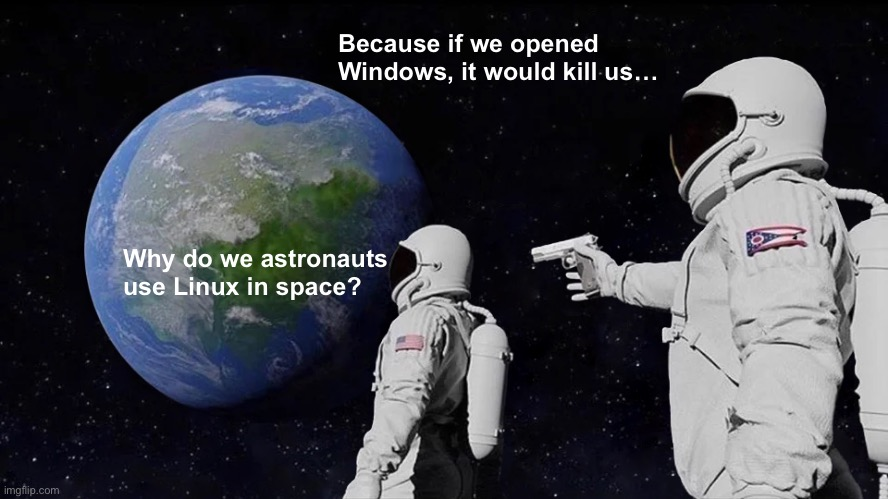
\includegraphics[width=7cm]{Meme_Space-Linux}
    \begin{exampleblock}<1->{Fun Fact}
        Linux im Weltall: ISS (Seit 1988) \& SpaceX (seit 2020).
    \end{exampleblock}

\end{frame}

\begin{frame}{Warum Linux?}
    
\includegraphics[width=7cm]{Meme_Server}

    \begin{exampleblock}{Fun Fact}
        96,3\% des Internets läuft auf Linux-Servern
    \end{exampleblock}
\end{frame}

\begin{frame}{Warum kein Linux?}
    \subsection{Warum kein Linux?}\label{subsec:warum-kein-linux?}

    \begin{itemize}
        \item Kein kompletter Microsoft-Office-Ersatz\pause
        \item Wenn man es einfach haben will (In Linux kann man sehr Tüfteln)\pause
        \item Mögliche Probleme beim Spielen
    \end{itemize}

\end{frame}

\begin{frame}{Distributionen}
    \subsection{Distributionen}\label{subsec:distributionen}

    Ein Großteil der Distributionen (Sorten) von Linux ist Teil dieser 3 "Familien":

    \begin{itemize}
        \item<2-> Arch
        \item<3-> Debian
        \item<4-> RHEL (Red Hat Enterprise Linux)
    \end{itemize}

    \vspace{0.5cm}
    \begin{exampleblock}<1->{Fun Fact}
        Die 500 Schnellsten Supercomputer der Welt laufen auf Linux
    \end{exampleblock}

\end{frame}


\begin{frame}{Desktop Umgebungen}
    \subsection{Desktop Umgebungen}\label{subsec:desktop-umgebungen}

    \begin{quote}
        Eine Desktop-Umgebung ist eine grafische Arbeits- bzw. Benutzerumgebung von Betriebssystemen in Form einer grafischen Shell [...]
    \end{quote}

    \pause

    \begin{itemize}
        \item Desktops sind auch nur eigenständige Software in einer Linux-Distribution\pause
        \item Leicht installierbar
    \end{itemize}

\end{frame}

\begin{frame}{Beispiele}
    \subsubsection{Beispiele}\label{subsubsec:beispiele}

    \href{https://opensource.com/article/20/5/linux-desktops}{Umfrage 2020 (opensource.com)}

    \begin{itemize}
        \item KDE Plasma (32\%)\pause
        \item Gnome (24\%)\pause
        \item XFCE (12\%)\pause
        \item Cinnamon (11\%)\pause
        \item sonst (21\%)
    \end{itemize}

\end{frame}

\begin{frame}{KDE Plasma}
    \subsubsection{KDE Plasma}\label{subsubsec:KDE-Plasma}

    \begin{tikzpicture}
        [remember picture, overlay, shift={(current page.north east)}]
        \node[anchor=north east,xshift=-.3cm,yshift=-2cm]{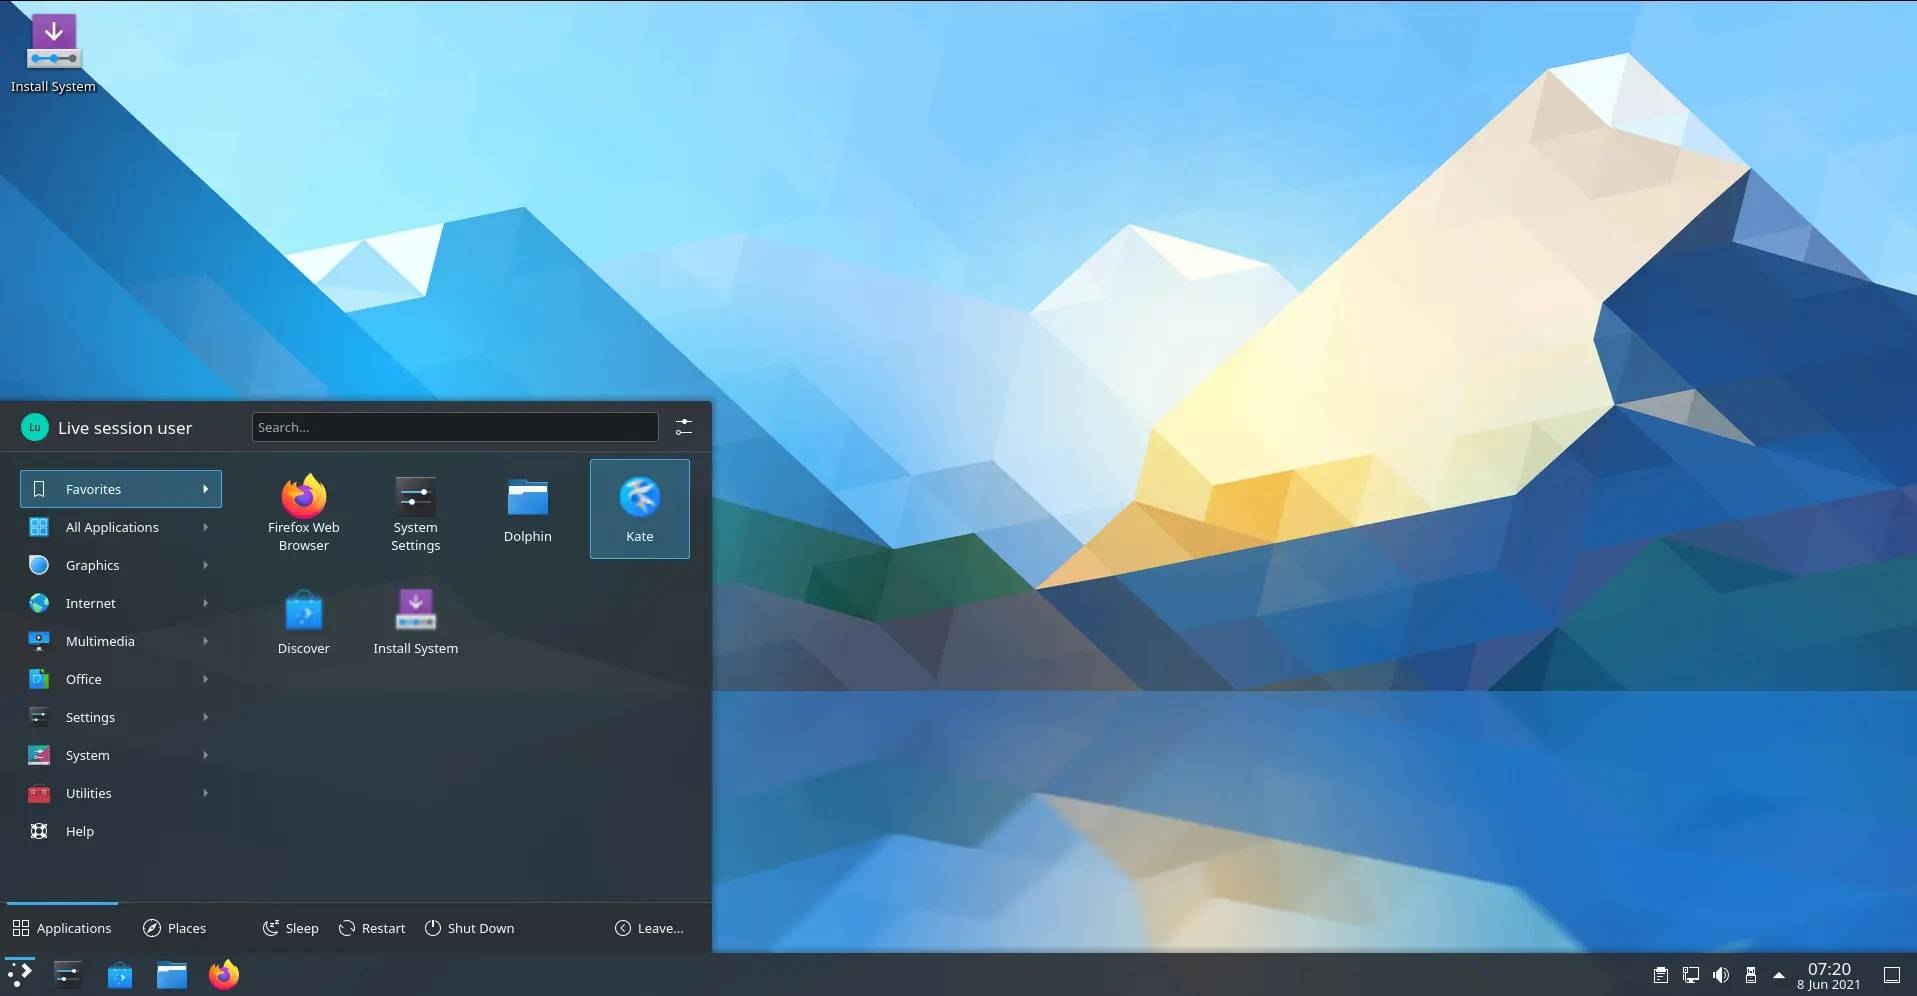
\includegraphics[width=12cm]{KDE-Plasma-Desktop}};
    \end{tikzpicture}

\end{frame}

\begin{frame}{Gnome}
    \subsubsection{Gnome}\label{subsubsec:Gnome}

    \begin{tikzpicture}
        [remember picture, overlay, shift={(current page.north east)}]
        \node[anchor=north east,xshift=-0.3cm,yshift=-2cm]{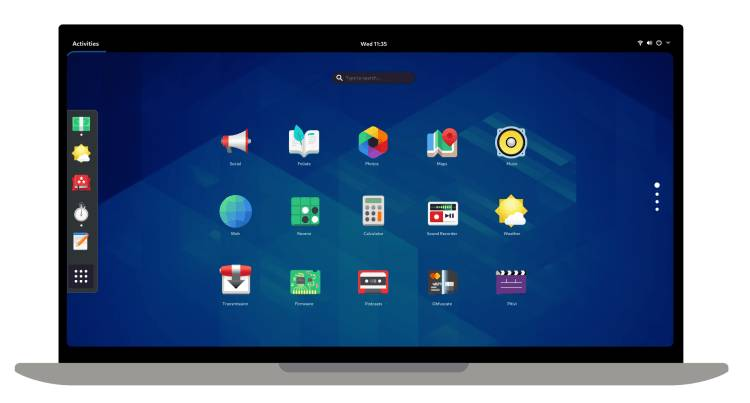
\includegraphics[width=12cm]{Gnome-Desktop}};
    \end{tikzpicture}

\end{frame}

\begin{frame}{XFCE}
    \subsubsection{XFCE}\label{subsubsec:XFCE}

    \begin{tikzpicture}
        [remember picture, overlay, shift={(current page.north east)}]
        \node[anchor=north east,xshift=-0.3cm,yshift=-1.7cm]{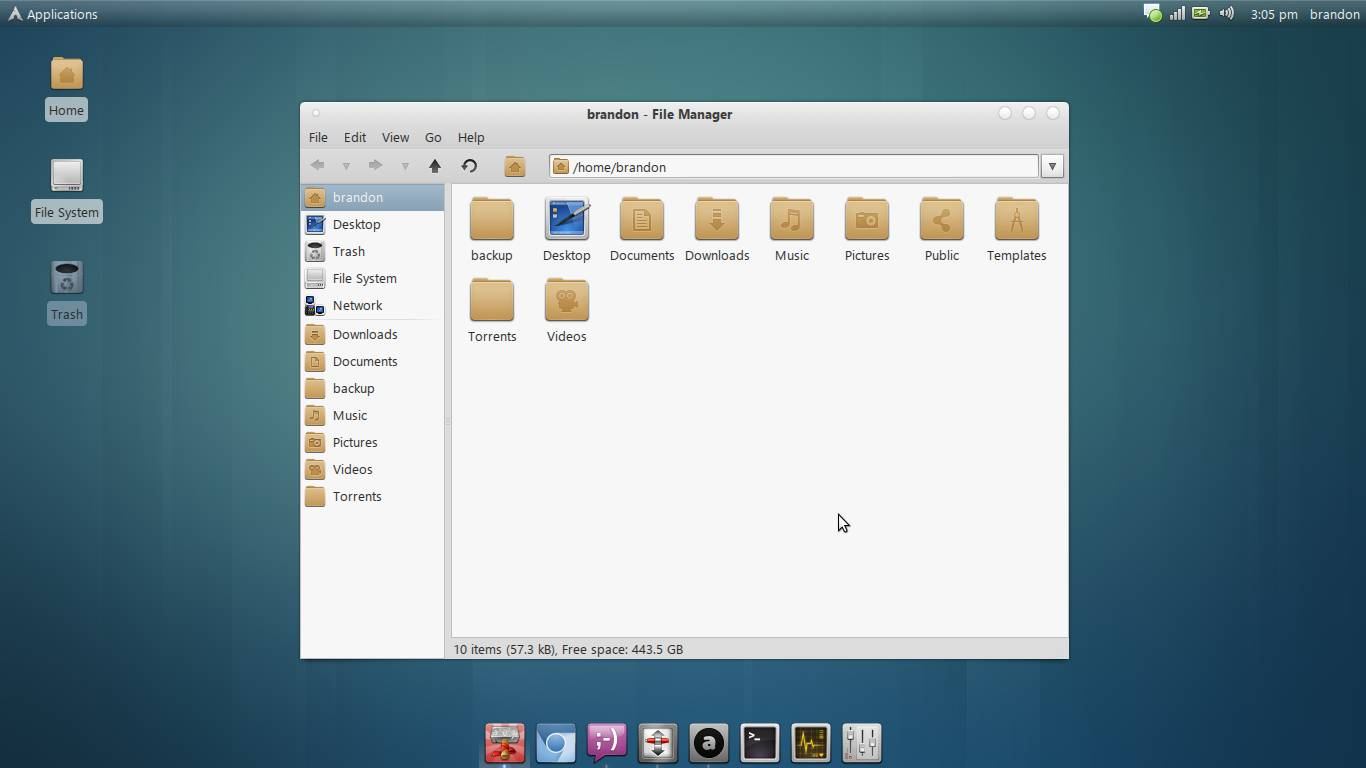
\includegraphics[width=12cm]{XFCE-Desktop}};
    \end{tikzpicture}

\end{frame}

\begin{frame}{Cinnamon}
    \subsubsection{Cinnamon}\label{subsubsec:Cinnamon}

    \begin{tikzpicture}
        [remember picture, overlay, shift={(current page.north east)}]
        \node[anchor=north east,xshift=-0.3cm,yshift=-1.7cm]{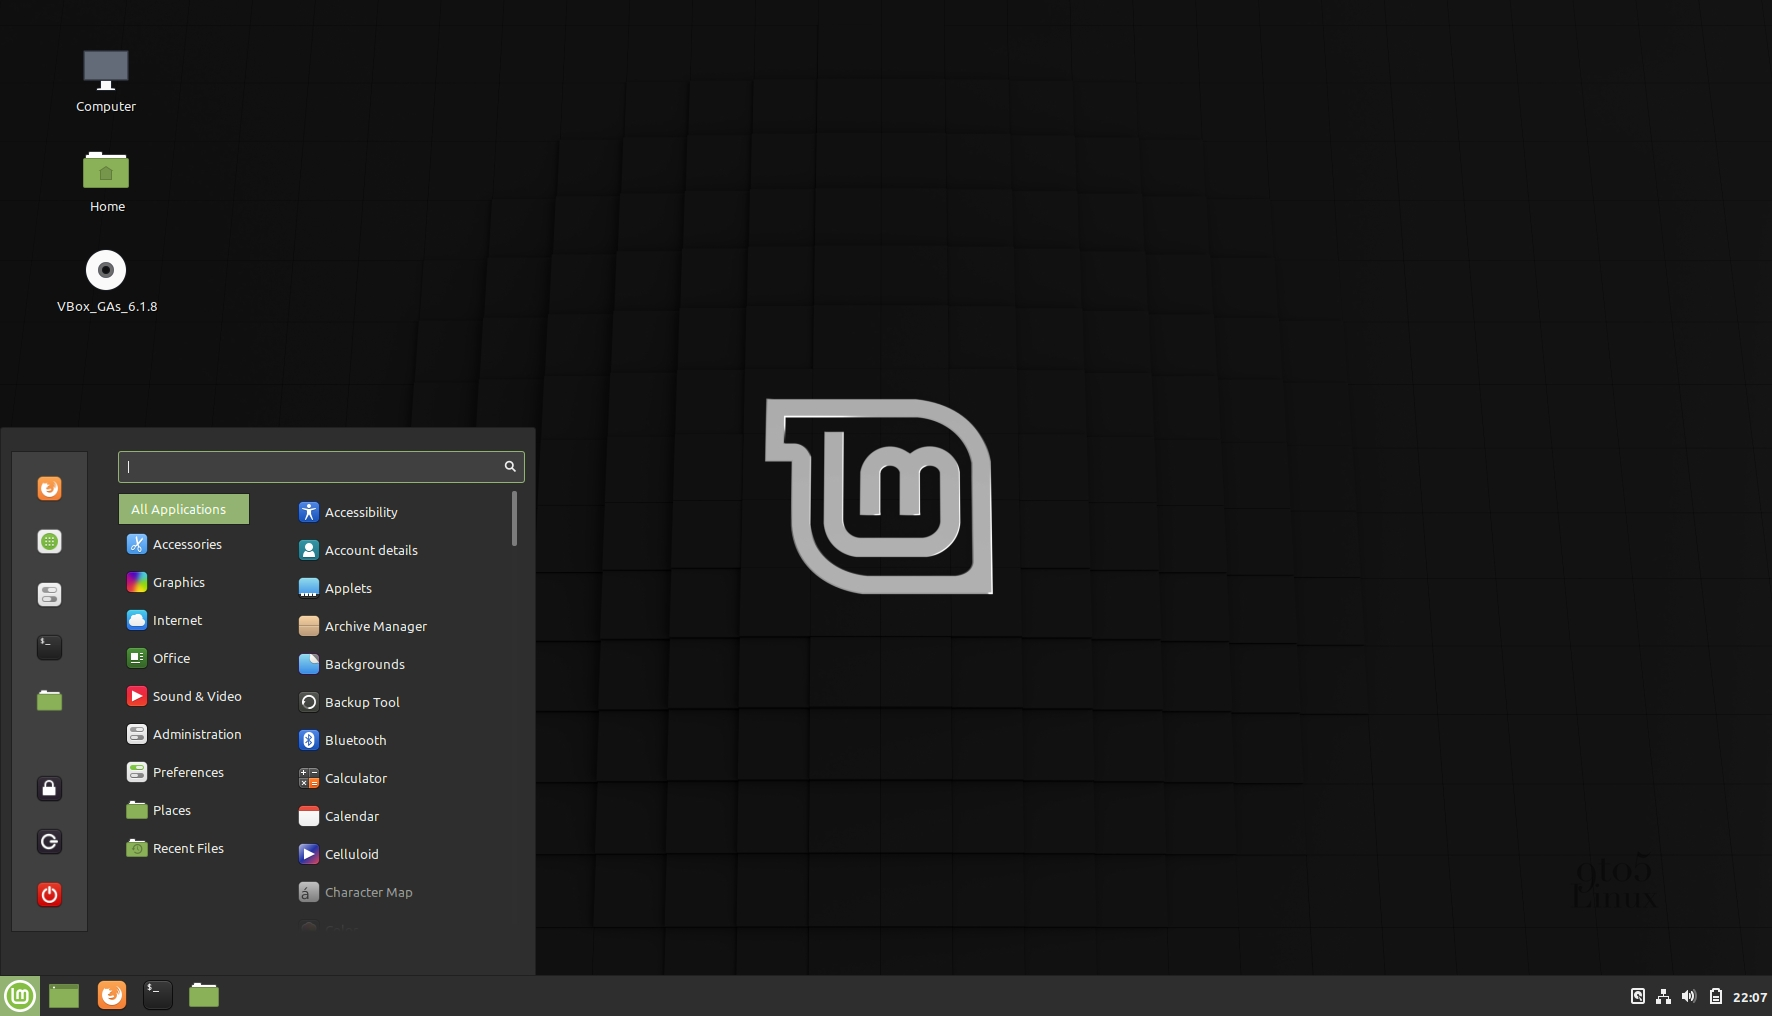
\includegraphics[width=12cm]{Mint-Desktop}};
    \end{tikzpicture}

\end{frame}


% Sources: https://www.forbes.com/sites/jasonevangelho/2019/02/14/5-gorgeous-examples-of-truly-customized-linux-desktops/
% Sources: https://github.com/vinceliuice/McMojave-kde
\begin{frame}{Other Desktops}
    \subsubsection{Other}\label{subsubsec:other}

    \begin{tikzpicture}
        [remember picture, overlay, shift={(current page.north east)}]
        \node[anchor=north east,xshift=-0.3cm,yshift=-1.7cm]{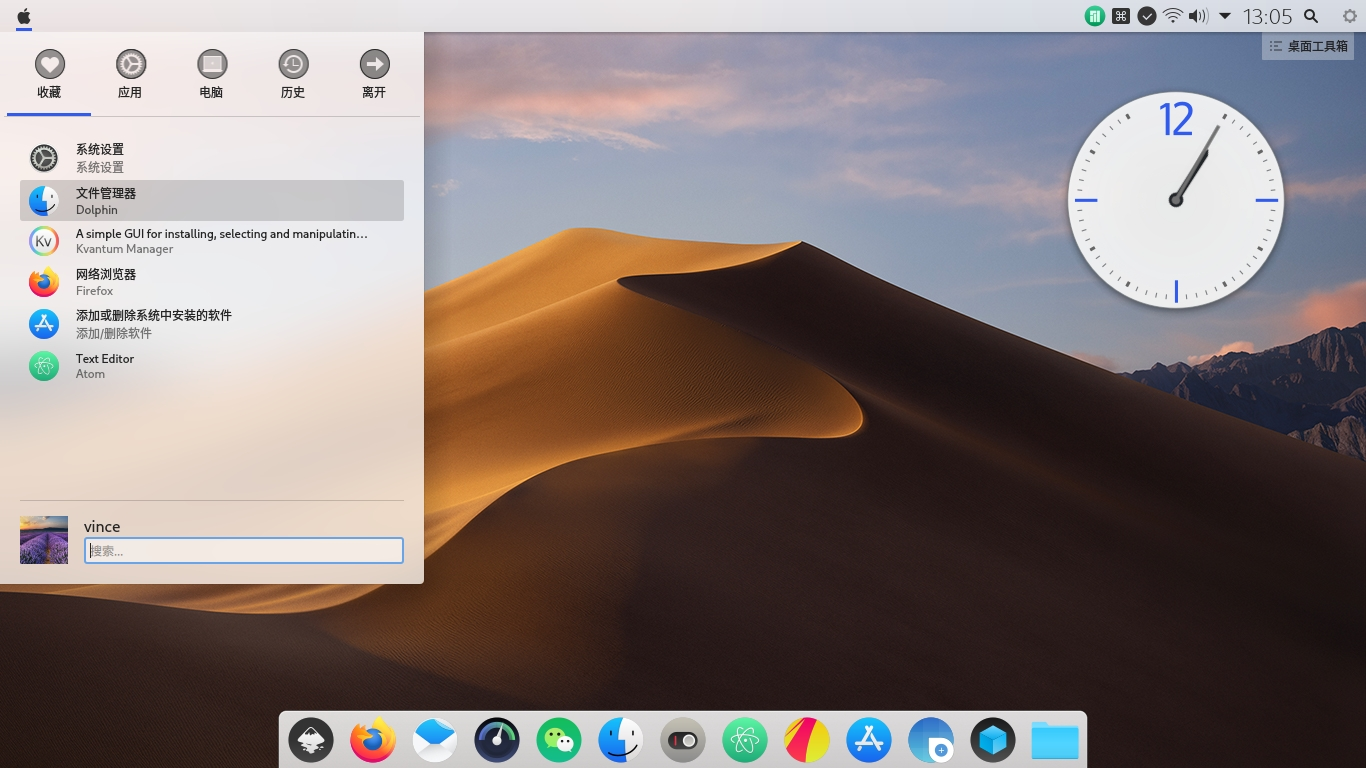
\includegraphics[width=12cm]{KDE-Desktop-MacOS}};
    \end{tikzpicture}

\end{frame}
\begin{frame}{Other Desktops}

    \begin{tikzpicture}
        [remember picture, overlay, shift={(current page.north east)}]
        \node[anchor=north east,xshift=-0.3cm,yshift=-1.7cm]{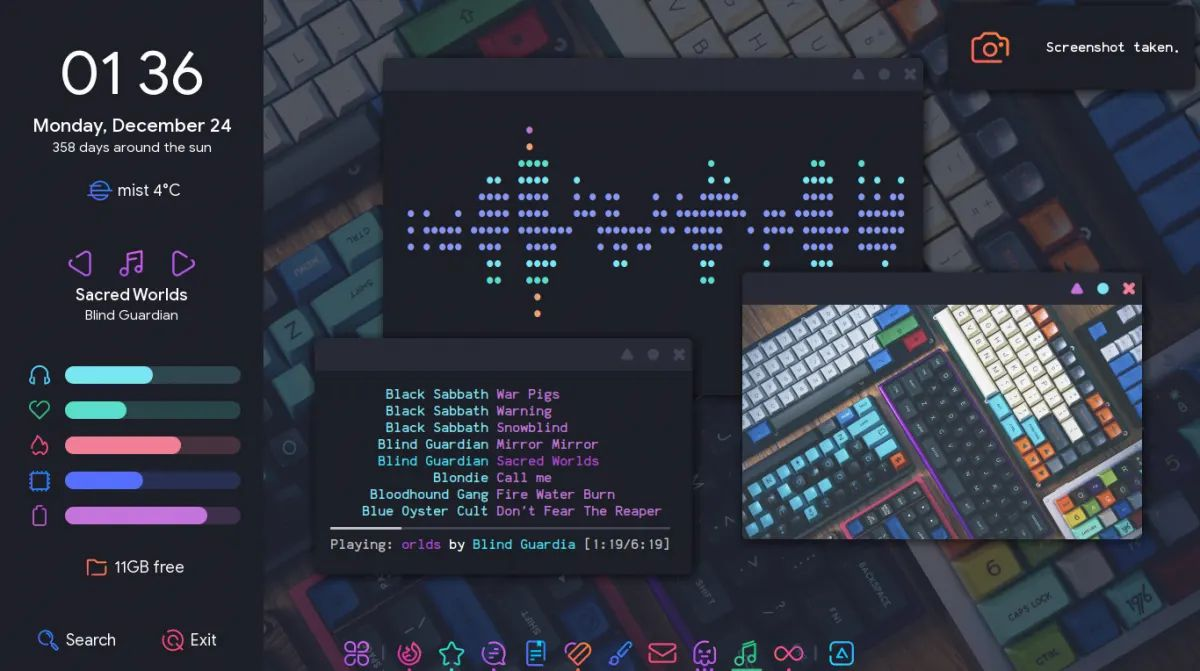
\includegraphics[width=12cm]{other-desktop-1}};
    \end{tikzpicture}

\end{frame}
\begin{frame}{Other Desktops}

    \begin{tikzpicture}
        [remember picture, overlay, shift={(current page.north east)}]
        \node[anchor=north east,xshift=-0.3cm,yshift=-1.7cm]{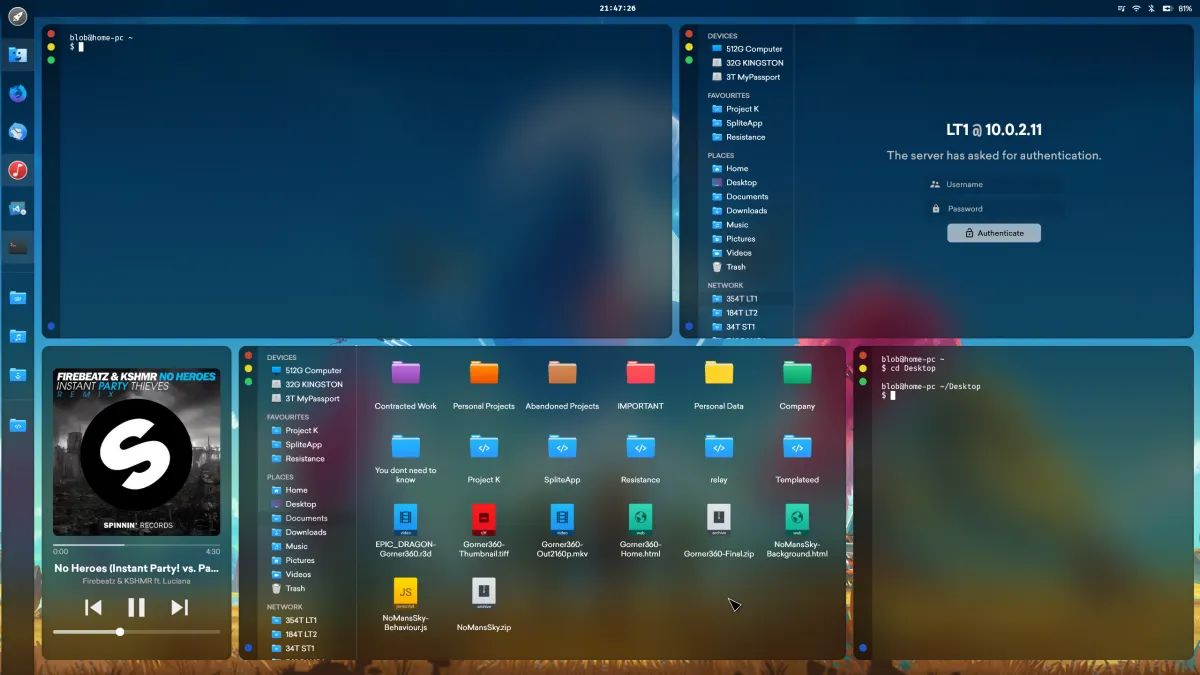
\includegraphics[width=12cm]{other-desktop-2}};
    \end{tikzpicture}

\end{frame}
\begin{frame}{Other Desktops}

    \begin{tikzpicture}
        [remember picture, overlay, shift={(current page.north east)}]
        \node[anchor=north east,xshift=-0.3cm,yshift=-1.7cm]{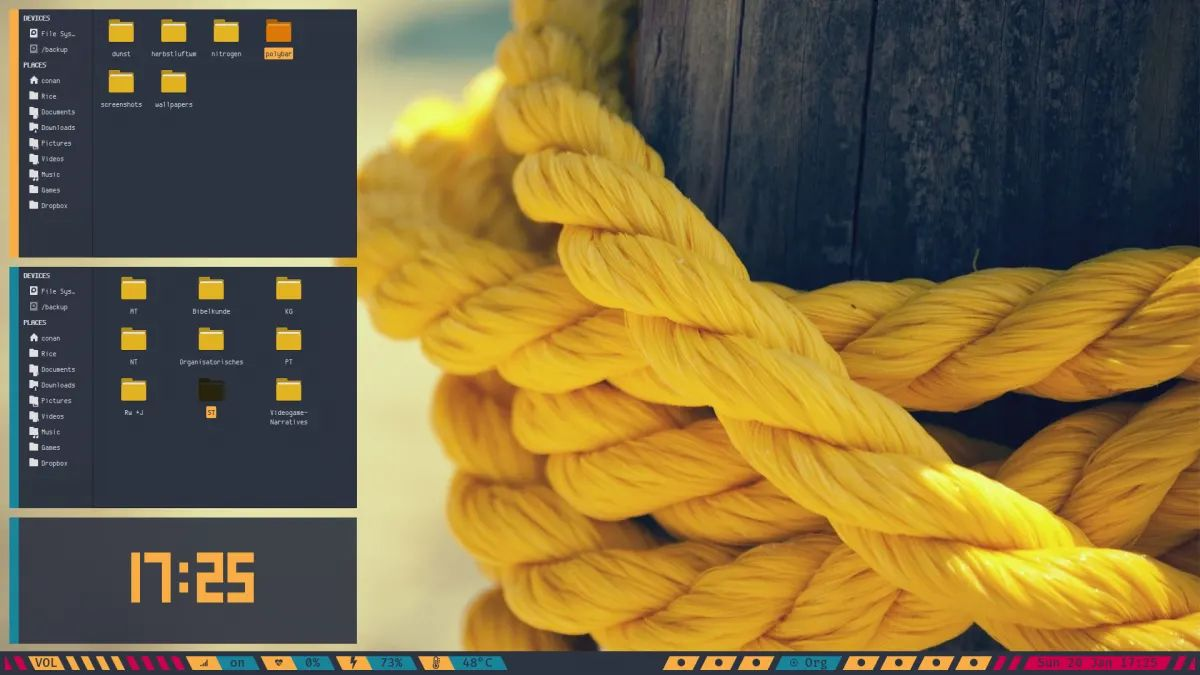
\includegraphics[width=12cm]{other-desktop-3}};
    \end{tikzpicture}

\end{frame}
    %! Author = paulsen
%! Date = 12.09.23

\begin{frame}{Installation}
    \section{Installation}\label{sec:installation}



\end{frame}

\begin{frame}{Linux Distributionen}

    Ein großteil der Distributionen (Sorten) von Linux ist Teil dieser 3 "Familien":

    \begin{itemize}
        \item Arch
        \item Debian
        \item RHEL (Red Hat Enterprise Linux)
    \end{itemize}



\end{frame}
    %! Author = paulsen
%! Date = 25.11.23

\begin{frame}{KDE Plasma}
    \section{KDE Plasma}\label{sec:KDE-Plasma}
\end{frame}

\begin{frame}{Einstellungen}
    \subsection{Plasma Einstellungen}\label{subsec:plasma-einstellungen}
    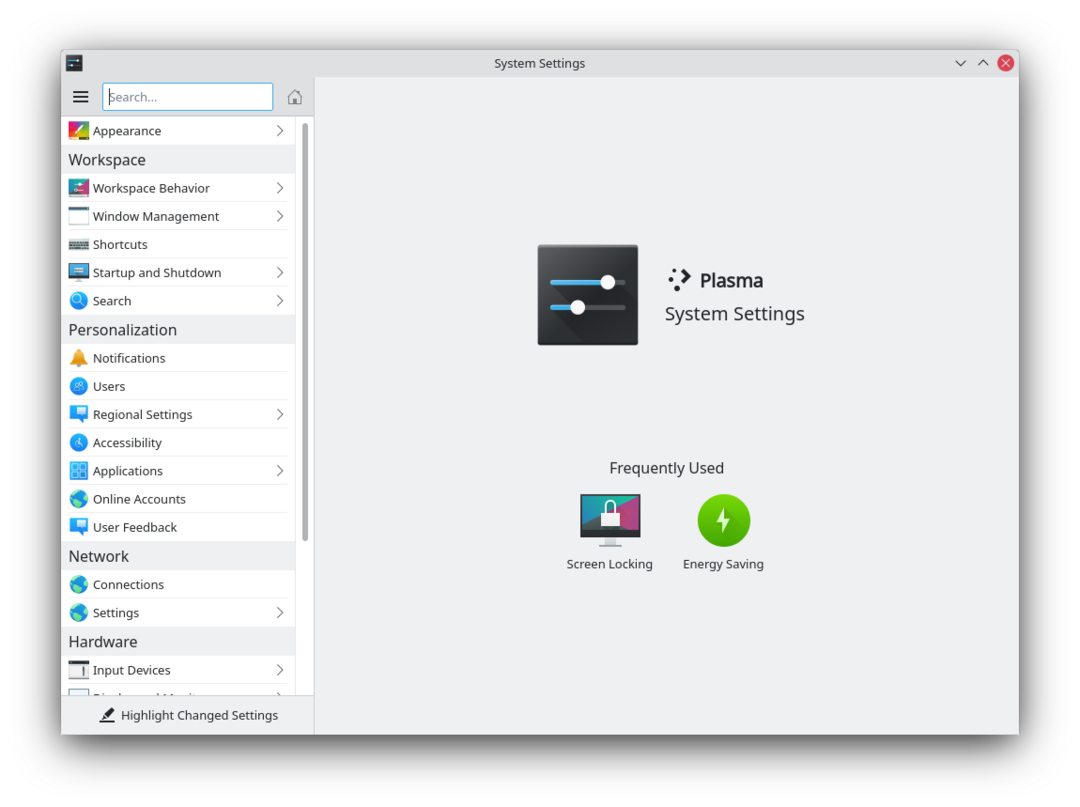
\includegraphics[width=11cm]{plasma-systemsettings}
\end{frame}

\begin{frame}{Einstellungen}

    \vspace{0.5cm}
    \begin{alertblock}{Aufgabe}
        Klicke dich durch die Einstellungen und erledige diese Aufgaben:

        \pause
        \begin{itemize}
            \item Ändere das Hintergrundbild\pause
            \item Ändere dein Nutzerpasswort\pause
            \item Verändere die systemweite Akzentfarbe\pause
            \item Erstelle mehrere Virtuelle Desktops\pause
            \item Verändere die Shortcuts zum Wechseln der Desktops
        \end{itemize}
    \end{alertblock}
\end{frame}

\begin{frame}{Widgets}
    \subsection{Widgets}\label{subsec:widgets}
    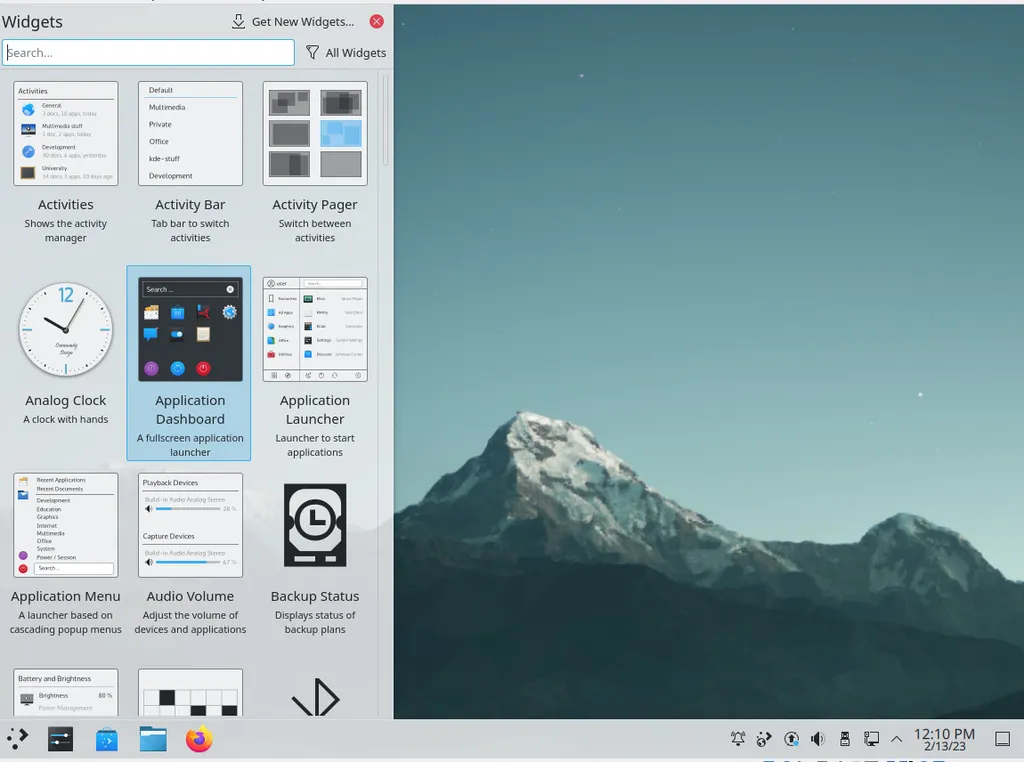
\includegraphics[width=11cm]{plasma-widgets}
\end{frame}

\begin{frame}{Widgets}

    Widgets sind kleine visuelle Anwendungen, die zur Anzeige von Informationen oder Shortcuts
    dienen.

    \pause

    \begin{itemize}
        \item Vor dem Desktophintergrund anzeigbar\pause
        \item Kann in die Desktop-Leiste eingefügt werden\pause
        \item Benutzer-Widgets können nachinstalliert werden
    \end{itemize}

    \pause
    \vspace{0.5cm}
    \begin{alertblock}{Aufgabe}
        \begin{itemize}
            \item Füge ein Mediaplayer-Widget in das Desktop-Panel ein.
            \item Verschiebe das Desktop-Panel an einen anderen Bildschirmrand und passe die Größe der Leiste an.
        \end{itemize}
    \end{alertblock}
\end{frame}

\begin{frame}{Vaults}
    \subsection{Vaults}\label{subsec:vaults}
    \begin{itemize}
        \item Verschlüsselte Ordner\pause
        \item Icon versteckt in Benachrichtigungsleiste\pause
        \item Ordner können mit der Cloud oder anderen Speichermedien synchronisiert und
        transportiert werden
    \end{itemize}

    \pause
    \vspace{0.5cm}
    \begin{alertblock}{Aufgabe}
        Erstelle einen mit Passwort verschlüsselten Ordner
    \end{alertblock}
\end{frame}
    %! Author = paulsenik
%! Date = 12.09.23

\begin{frame}{Software}
    \section{Software}\label{sec:software}
\end{frame}


\begin{frame}{Pakete}
    \subsection{Pakete}\label{subsec:pakete}

    Was sind (Software-)Pakete?
    \pause

    \vspace{0.5cm}
    \begin{quote}
        Eine Paketverwaltung ermöglicht die komfortable Verwaltung von Software, die in Form von Programmpaketen vorliegt.
    \end{quote}
    \pause

    \begin{itemize}
        \item Pakete sind an einer Zentralen Stelle (auch "Repository") hinterlegt\pause
        \item Ermöglicht strukturierte Updates\pause
        \item Kein Linux-Einheitliches Paketformat
    \end{itemize}
\end{frame}

\begin{frame}{Pakete}
    \subsection{Varianten}\label{subsec:varianten}

    Die Installation von Programmen/Paketen erfolgt über unterschiedliche Paket-Manager.

    \begin{enumerate}
        \item<2-> Distributions-Spezifische Paketformate
        \item<3-> Unabhängige Containerformate
        \item<4-> Sonstiges: Appimage, Nativ, Compiliert mit Sourcecode
    \end{enumerate}

    \vspace{0.5cm}
    \begin{exampleblock}<1->{Fun Fact}
        Android hat "APK" als einheitliches Paketformat
    \end{exampleblock}

\end{frame}

\begin{frame}{Spezifische Paketformate}
    \subsubsection{}\label{subsubsec:spezifische-formate}

    \minipage{0.49\textwidth}
        Distributionsspezifische Paketmanager die mit System-Rechten laufen:
        \begin{itemize}
            \item<2-> APT
            \item<3-> PACMAN
            \item<4-> DNF
            \item<5-> \ldots
        \end{itemize}
    \endminipage\hfill
    \minipage{0.49\textwidth}
        
\includegraphics[width=\linewidth]{Meme_Uninstall-Bootloader}
    \endminipage\hfill
\end{frame}

\begin{frame}{Containerformate}
    \subsubsection{}\label{subsubsec:containerformate}

    Laufen System-Unabhängig und meistens auf Benutzer-Level
    \pause

    \begin{itemize}
        \item Flatpak\pause
        \item Snap\pause
        \item Docker
    \end{itemize}

\end{frame}

\begin{frame}{Sonstige Paketformate}
    \subsubsection{}\label{subsubsec:sonstige-paketformate}

    \begin{itemize}
        \item Appimage: Einzelne Datei beinhaltet die Anwendung und alles was es benötigt\pause
        \item Nativ: Anwendungs-Version ist nur für spezifische Geräteart (ARM-Prozessor, IOS, x86)\pause
        \item Quellcode: Beim Benutzer wird eine (seinem System) zugeschnittene Anwendung erstellt.
    \end{itemize}

\end{frame}

\begin{frame}{Software Installation}
    \subsection{Installation}\label{subsec:installation}

    \begin{itemize}
        \item Installation Grafisch oder über Konsole möglich\pause
        \item "Discover" kann Programme verschiedener Paketarten installieren
    \end{itemize}

\end{frame}

\begin{frame}{Discover}
    \subsubsection{Discover}\label{subsubsec:discover}

    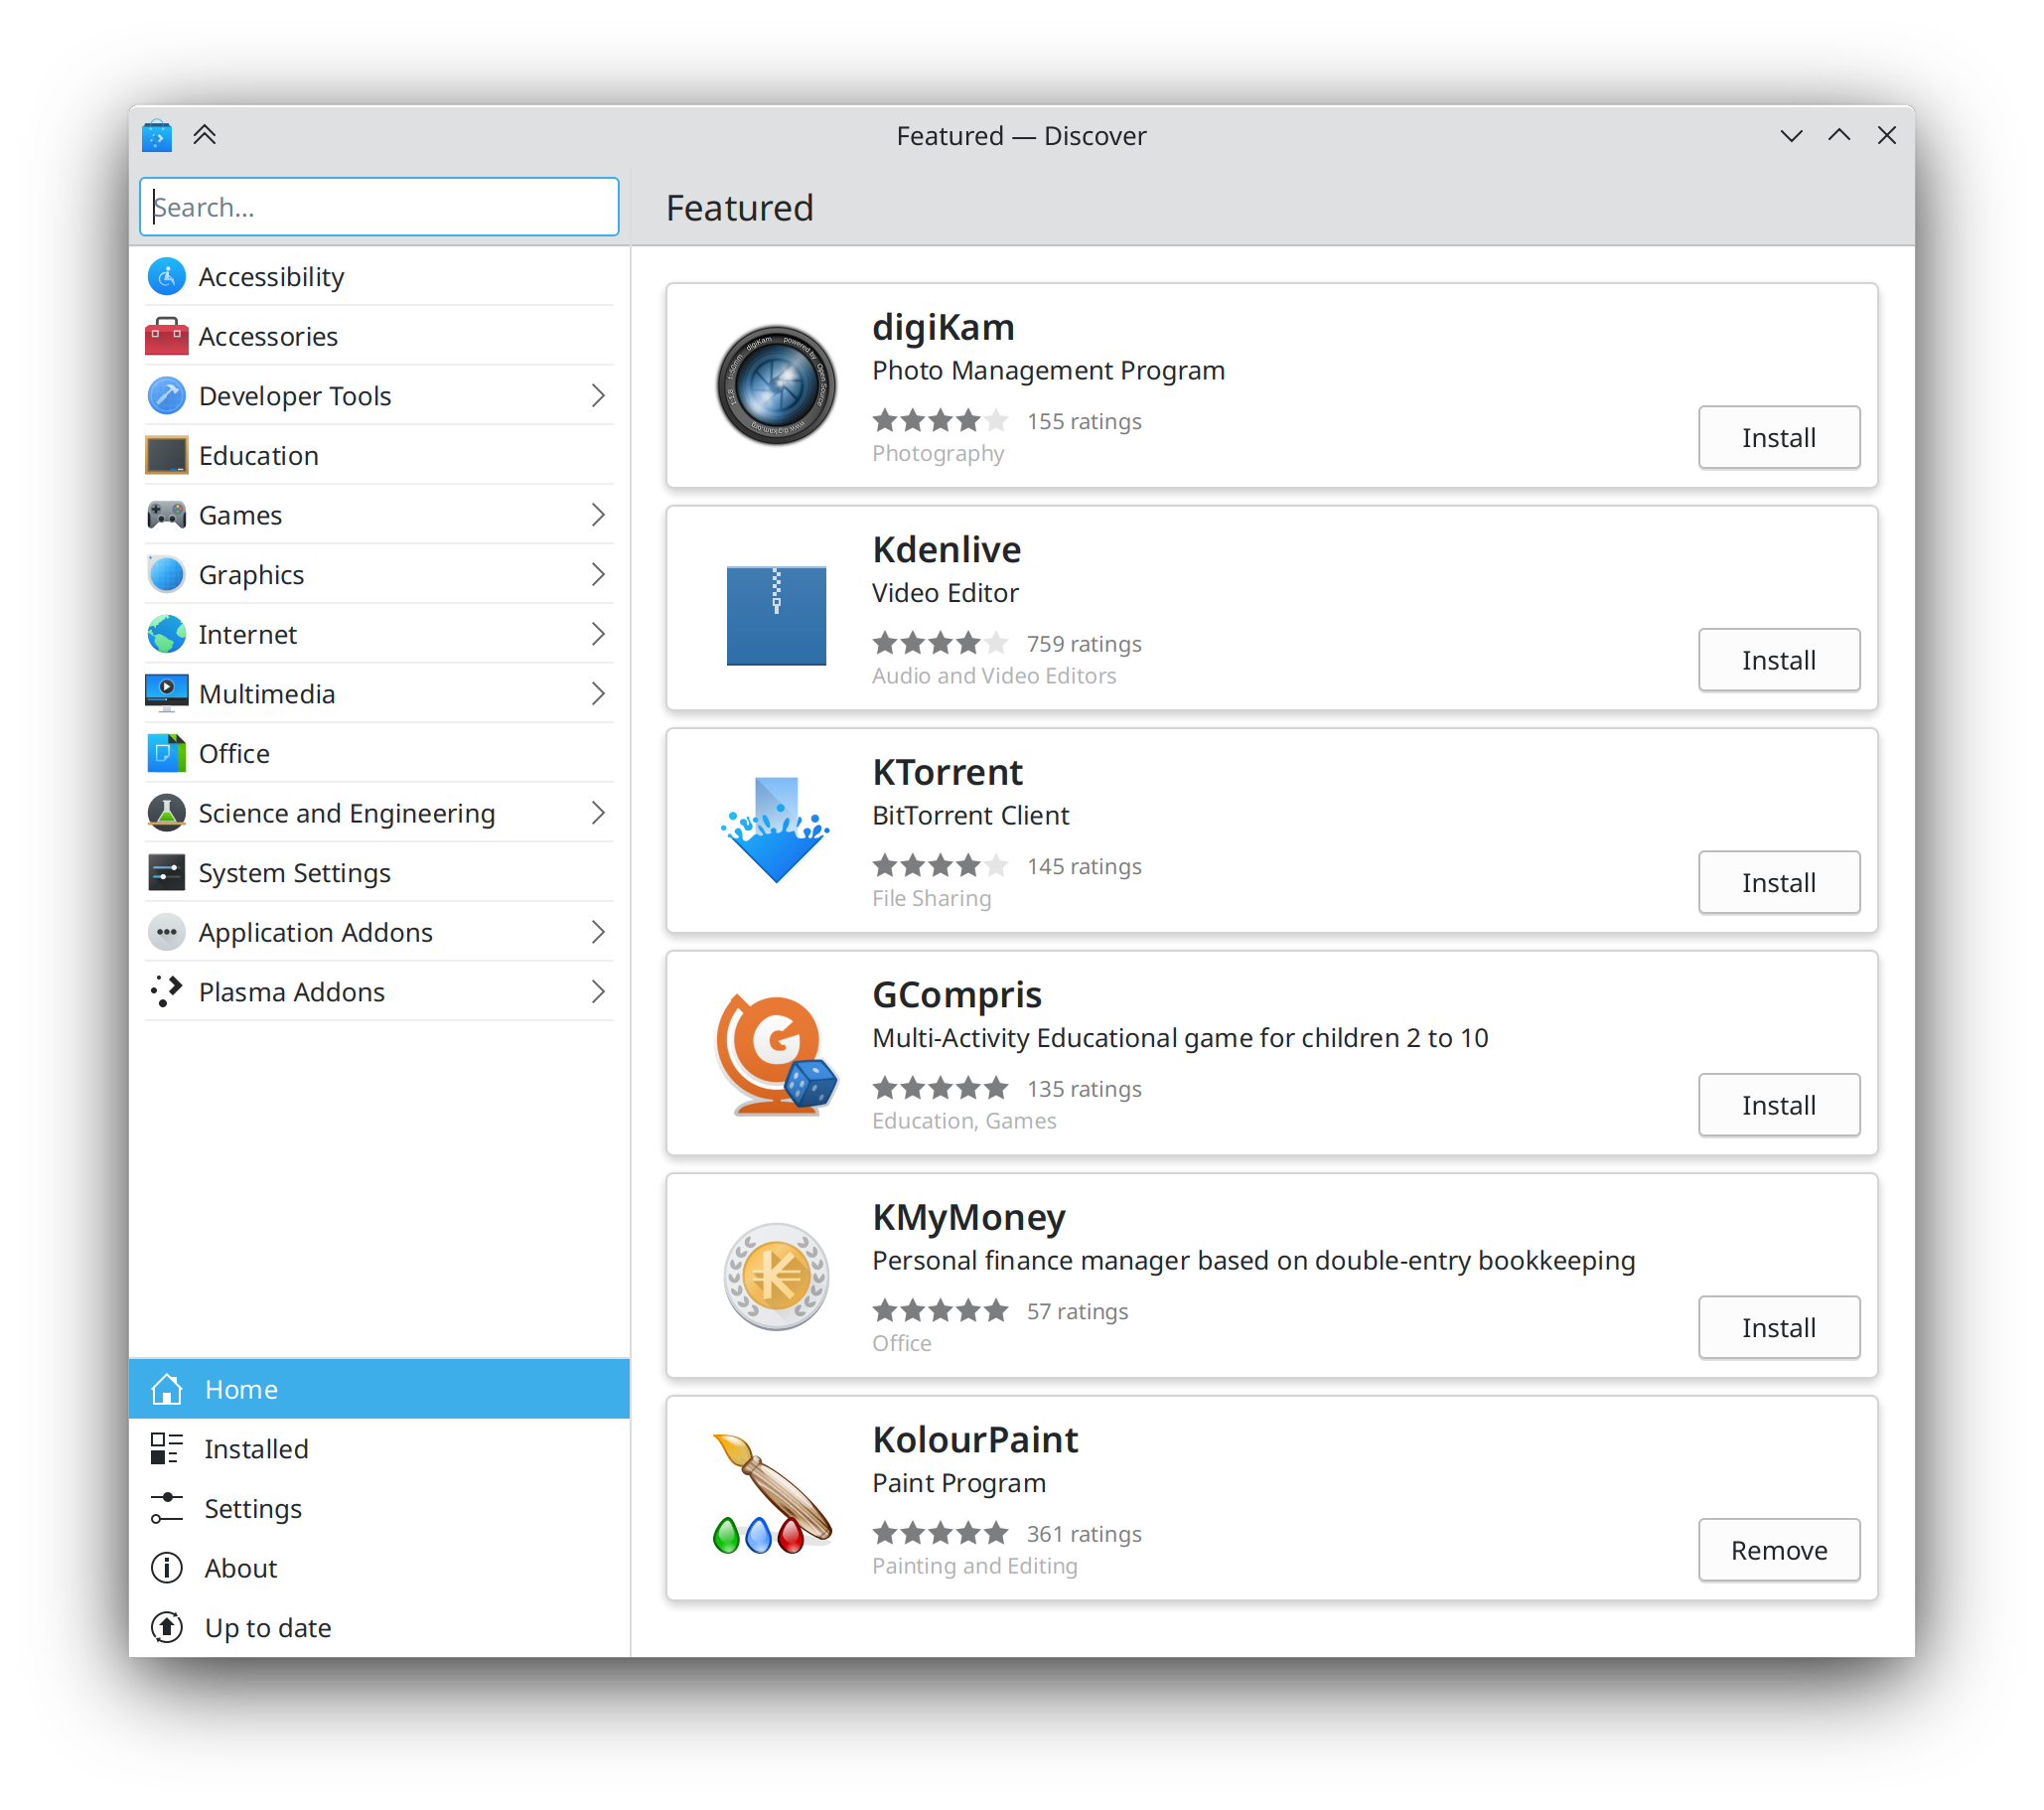
\includegraphics[width=10cm]{plasma-discover}
\end{frame}

\begin{frame}{Discover}

    \vspace{0.5cm}
    \begin{alertblock}{Aufgabe}
        Installiere folgende Programme:
        \begin{itemize}
            \item OnlyOffice
            \item Xournal++
        \end{itemize}
    \end{alertblock}
    \pause

    \vspace{0.5cm}
    \begin{alertblock}{Aufgabe}
        Aktualisiere dein System.
    \end{alertblock}

\end{frame}

\begin{frame}{Office}

    \begin{itemize}
        \item OnlyOffice: All-In-One Microsoft-Office Ersatz\pause
        \item Xournal++: Notizen\pause
        \item Okular: PDF-Reader und Formulare\pause
        \item PDFPC: Presenter
    \end{itemize}

\end{frame}

\begin{frame}{Office}
    \vspace{0.5cm}
    \begin{alertblock}{Aufgabe}
        \begin{enumerate}
            \item Erstelle ein Office-Dokument mithilfe von OnlyOffice.\pause
            \item Exportiere dieses Dokument als PDF.\pause
            \item Mache dich mit Xournal++ vertraut und unterschreibe das Dokument.\pause
            \item Exportiere das unterschriebene Dokument wieder als PDF.\pause
            \item Öffne das PDF-Dokument mit Okular und überprüfe das Dokument.
        \end{enumerate}
    \end{alertblock}
\end{frame}
    %! Author = paulsenik
%! Date = 12.09.23

\begin{frame}{Die Konsole}
    \section{Die Konsole}\label{sec:die-konsole}
\end{frame}

\begin{frame}{Die "Wurzel"}

    \begin{quote}
        Die Wurzel (/), auch "root" genannt, ist der Ursprung des Dateisystems.
    \end{quote}
    \pause

    \begin{itemize}
        \item Die Wurzel ist ähnlich zum "C:\textbackslash"-Pfad in Windows\pause
        \item In "/home" leben alle Nutzer und ihre Daten\pause
        \item Dateisystem beginnt hier
    \end{itemize}

\end{frame}

\begin{frame}{Das Dateisystem}
    \subsection{Dateisystem}\label{subsec:dateisystem}

    \begin{quote}
        Alles in Linux ist eine Datei!?
    \end{quote}


    \begin{itemize}
        \item<2-> Konfigurationen (/etc)
        \item<3-> Commands (/bin)
        \item<4-> Geräte (/dev)
        \item<5-> Speichermedien (/media /mnt)
    \end{itemize}

    \vspace{0.5cm}
    \begin{exampleblock}{Fun Fact}<1->
        Dateien mit Punkt am Anfang (.bashrc .git) werden im Explorer standardmäßig versteckt.
    \end{exampleblock}
\end{frame}

\begin{frame}{Die Shell}
    \subsection{Die Shell}\label{subsec:die-shell}

    Die Shell ermöglicht direkten Zugriff auf das Betriebssystem.
    \pause

    \begin{itemize}
        \item Das mächtigste Werkzeug in Linux\pause
        \item Navigation durch das Dateisystem\pause
        \item Ausführen von System-Befehlen\pause
        \item Anzeige von Informationen
    \end{itemize}
    \pause

    \vspace{0.5cm}
    
\includegraphics[width=3cm]{plasma-konsole}
    \pause

    \vspace{0.5cm}
    \begin{alertblock}{Aufgabe}
        Öffne die Konsole und führe "whoami" aus.
    \end{alertblock}

\end{frame}

\begin{frame}{Befehle}
    \subsection{Befehle}\label{subsec:befehle}

    Ein Befehl besteht aus bis zu drei Teilen:
    \pause

    \begin{enumerate}
        \item Befehlsname\pause
        \item Optionen\pause
        \item Argumente
    \end{enumerate}
    \pause

    \vspace{0.5cm}
    \begin{exampleblock}{Beispiel}
        \$ ls -la /home/Nutzer/Dokumente
    \end{exampleblock}
    \pause

    \vspace{0.5cm}
    \begin{alertblock}{Aufgabe}
        Probiere diesen Befehl mit und ohne den Optionen bzw Argumenten.
    \end{alertblock}

\end{frame}

\begin{frame}{Navigation}
    \subsection{Navigation}\label{subsec:navigation}

    Wie navigiere ich durch das Dateisystem?
    \pause

    \textrightarrow "cd" wechselt den aktuellen Ordner
    \pause

    \begin{itemize}
        \item[\$] cd Ordnername\pause
        \item[\$] cd ..\pause
        \item[\$] cd
    \end{itemize}
    \pause

    \vspace{0.5cm}
    \begin{alertblock}{Aufgabe}
        Navigiere zum Ordner mit den Kurs-Dokumenten.
    \end{alertblock}
    \pause

    Platzhalter bei Befehlen:

    \begin{itemize}
        \item \textasciitilde\space für das Nutzer-Verzeichnis\pause
        \item . für den aktuellen Ordner\pause
        \item .. für den Überordner
    \end{itemize}

\end{frame}

\begin{frame}{Befehlshilfe}
    \subsection{Befehlshilfe}\label{subsec:befehlshilfe}

    Hilfe ich kenne diesen Befehl nicht!
    \pause

    \textrightarrow Zur Hilfe für unbekannte Befehle gibt es "man".
    \pause

    \vspace{0.5cm}
    \begin{alertblock}{Aufgabe}
        Ausprobieren:

        \begin{itemize}
            \item[\$] man man\pause
            \item[\$] man ls\pause
            \item[\$] man
        \end{itemize}
    \end{alertblock}
    \pause

    Wie komme ich da jetzt raus?
    \pause

    \textrightarrow Q drücken

\end{frame}

\begin{frame}{Textbearbeitung}
    \subsection{Textbearbeitung}\label{subsec:textbearbeitung}

    "nano" ist ein CLI-Programm zum Bearbeiten und Erstellen von Dateien.
    \pause

    \begin{itemize}
        \item CTRL + X zum Beenden\pause
        \item CTRL + O zum Speichern\pause
        \item CTRL + C zum Abbrechen des Speicherprozesses
    \end{itemize}
    \pause

    \vspace{0.5cm}
    \begin{alertblock}{Aufgabe}
        \begin{itemize}
            \item Erstelle eine Datei mit nano\pause
            \item[\$] nano test.txt
        \end{itemize}
    \end{alertblock}

\end{frame}

\begin{frame}{Dateien}
    \subsection{Dateien}\label{subsec:dateien}

    Umgang mit Dateien:
    \pause

    \begin{itemize}
        \item Bearbeiten: \$ nano datei.txt\pause
        \item Inhalt: \$ cat datei.txt\pause
        \item Entfernen: \$ rm datei.txt\pause
        \item Kopieren: \$ cp datei.txt neu.txt\pause
        \item Verschieben: \$ mv datei.txt neu.txt
    \end{itemize}
    \pause

    \vspace{0.5cm}
    \begin{exampleblock}{Tipp}
        Der "man"-Befehl kann beim Verständnis helfen.
    \end{exampleblock}

\end{frame}

\begin{frame}{Dateien - Übung}
    \subsubsection{Übung}\label{subsubsec:übung}

    \begin{alertblock}{Aufgaben}
        \begin{enumerate}
            \item Kannst du die Datei ".bashrc" finden?\pause
            \item Wann wurde die Datei zuletzt verändert?\pause
            \item Kopiere die Test-Datei in den Benutzerordner.\pause
            \item Benenne die Datei in "Ich-Kann-Bash" um.\pause
            \item Entferne die alte Datei.
        \end{enumerate}
    \end{alertblock}
    \pause

    \vspace{0.5cm}
    \begin{alertblock}{Extra}
        Informiere dich mithilfe von "man apt" über den APT-Befehl
    \end{alertblock}

\end{frame}

\begin{frame}{APT}
    \subsection{APT}\label{subsec:apt}

    APT ist der wichtigste Paket-Manager auf Debian/Ubuntu Systemen.
    \pause

    \textrightarrow Über shell steuerbar.
    \pause

    \begin{itemize}
        \item[\$] man apt\pause
        \item[\$] apt list \textminus\textminus installed\pause
        \item[\$] apt update\pause
        \item[\$] apt upgrade\pause
        \item[\$] apt install Programm\pause
        \item[\$] apt remove Programm
    \end{itemize}

\end{frame}

\begin{frame}{Sudo}
    \subsection{Sudo}\label{subsec:sudo}

    \begin{quote}
        Wie sagen wir, wenn wir höflich um Erlaubnis fragen?
    \end{quote}
    \pause

    \textrightarrow Richtig! "sudo"
    \pause

    \begin{itemize}
        \item Superuser do!\pause
        \item Lässt Admin-Befehle zu\pause
        \item Zum Schutz des "normalen" Nutzers\pause
        \item Mit Passwort-Eingabe verbunden\pause
        \item Steht direkt vor dem eigentlichen Befehl
    \end{itemize}
    \pause

    \vspace{0.5cm}
    \begin{exampleblock}{Beispiel}
        \begin{itemize}
            \item[\$] sudo apt install firefox
        \end{itemize}
    \end{exampleblock}

\end{frame}

\begin{frame}{Sudo}
    \begin{alertblock}{Aufgabe}
        Erledige diese Dinge mit der Shell:
        \begin{enumerate}
            \item Installiere "pdfpc"\pause
            \item Entferne "okular"\pause
            \item Aktualisiere dein System
        \end{enumerate}
    \end{alertblock}
\end{frame}

\begin{frame}{CLI Programme}
    \subsection{CLI Programme}\label{subsec:cli-programme}

    \begin{alertblock}{Aufgabe}
        Präsentiere PDFs von der Konsole aus:
        \begin{itemize}
            \item[\$] pdfpc präsentation.pdf\pause
            \item "TAB" zur Übersicht\pause
            \item "1,2,3,4" zum Modus wechseln\pause
            \item "CTRL + Q" zum Beenden
        \end{itemize}
    \end{alertblock}
    \pause

    Weitere CLI-Programme: nano, vim, man, htop ...

\end{frame}

    %! Author = paulsen
%! Date = 12.09.23


\begin{frame}{Probleme \& Fragen}
    \section{Probleme \& Fragen}\label{sec:probleme-&-fragen}

    TODO


\end{frame}
    %! Author = paulsen
%! Date = 12.09.23

\begin{frame}{Schluss}
    \section{Schluss}\label{sec:schluss}
\end{frame}

\begin{frame}{Fragen}
    \subsection{Fragen}\label{subsec:Fragen}

    Fragen:

    \begin{itemize}
        \item Bezüglich Linux allgemein?
        \item Unklarheiten?
        \item Fehlende Themen?
        \item Verbesserungswünsche?
    \end{itemize}

\end{frame}

\begin{frame}{Feedback}
    \subsection{Feedback}\label{subsec:feedback}

    \vspace{0.5cm}
    \begin{alertblock}{Aufgabe}
        Bitte den Feedbackbogen in Stud.IP ausfüllen.
        \linebreak
        Danke :)
    \end{alertblock}

\end{frame}

    \begin{frame}[standout]
        Danke
    \end{frame}

\end{document}